\section{Deconstruction}
\label{sec:chapter_4_section_3}

Il progetto \emph{Deconstruction} nasce con l'idea di fare delle previsioni
sui costi di demolizione e smaltimento dei materiali di scarto degli edifici (Figura ~\ref{fig:augmented}).
Il progetto ha lo scopo di promuovere l'uso di strumenti informatici semplificati per sostenere la decostruzione.
In particolare, fornisce un modellazione geometrica semplificata dell'edificio permettendo l'integrazione di una descrizione
semantica delle componenti e dei loro materiali.
La realtà Virtuale/Aumentata aiuta a superare le difficoltà amministrative, a condizione di avere una
corretta identificazione dei rifiuti prodotti. Questo approccio aumenta l'adozione di comportamenti virtuosi,
cioè il recupero e riutilizzo.
In particolare, una modellazione geometrica dell'edificio permette di individuare:
\begin{itemize}
  \item  costi/entrate derivanti da alternative di riciclo/riutilizzo, invece di smaltimento;
  \item  la composizione e l'integrazione di informazioni utili per la pianificazione delle attività di costruzione;
  \item  realizzazione delle soglie di riutilizzo/recupero previsti dalla normativa;
  \item  capacità di confrontare economicamente diverse opzioni.
\end{itemize}

Il progetto ha avuto inizio prendendo in considerazione il sistema SMARTWaste~\cite{smartWaste}.
Questo approccio permette di ricavare stime delle quantità di materiali, fornendo una descrizione del tipo di edificio
e la zona in cui è stato costruito. Con queste informazioni, si fornisce una rappresentazione aggregata dei dati di
interesse sono riempiendo automaticamente delle form.
Il framework \emph{Metior} nel contesto della decostruzione al contrario fornisce sia una modellazione geometrica di sottosistemi
e componenti edilizi e un annotazione semantica con materiali da costruzione, come una sorta di \emph{BIM semplificato}.
È un dato di fatto, che il settore edile nazionale è fortemente eterogeneo, necessita di una modellazione
dettagliata per ottenere delle informazioni sufficientemente accurate.
Un punto di vista di questo approccio è il carattere iterativo incrementale, in cui ogni fase di modellazione può essere
seguita da una validazione dei costi parziali.

\begin{figure}[htbp] %  figure placement: here, top, bottom, or page
   \centering
   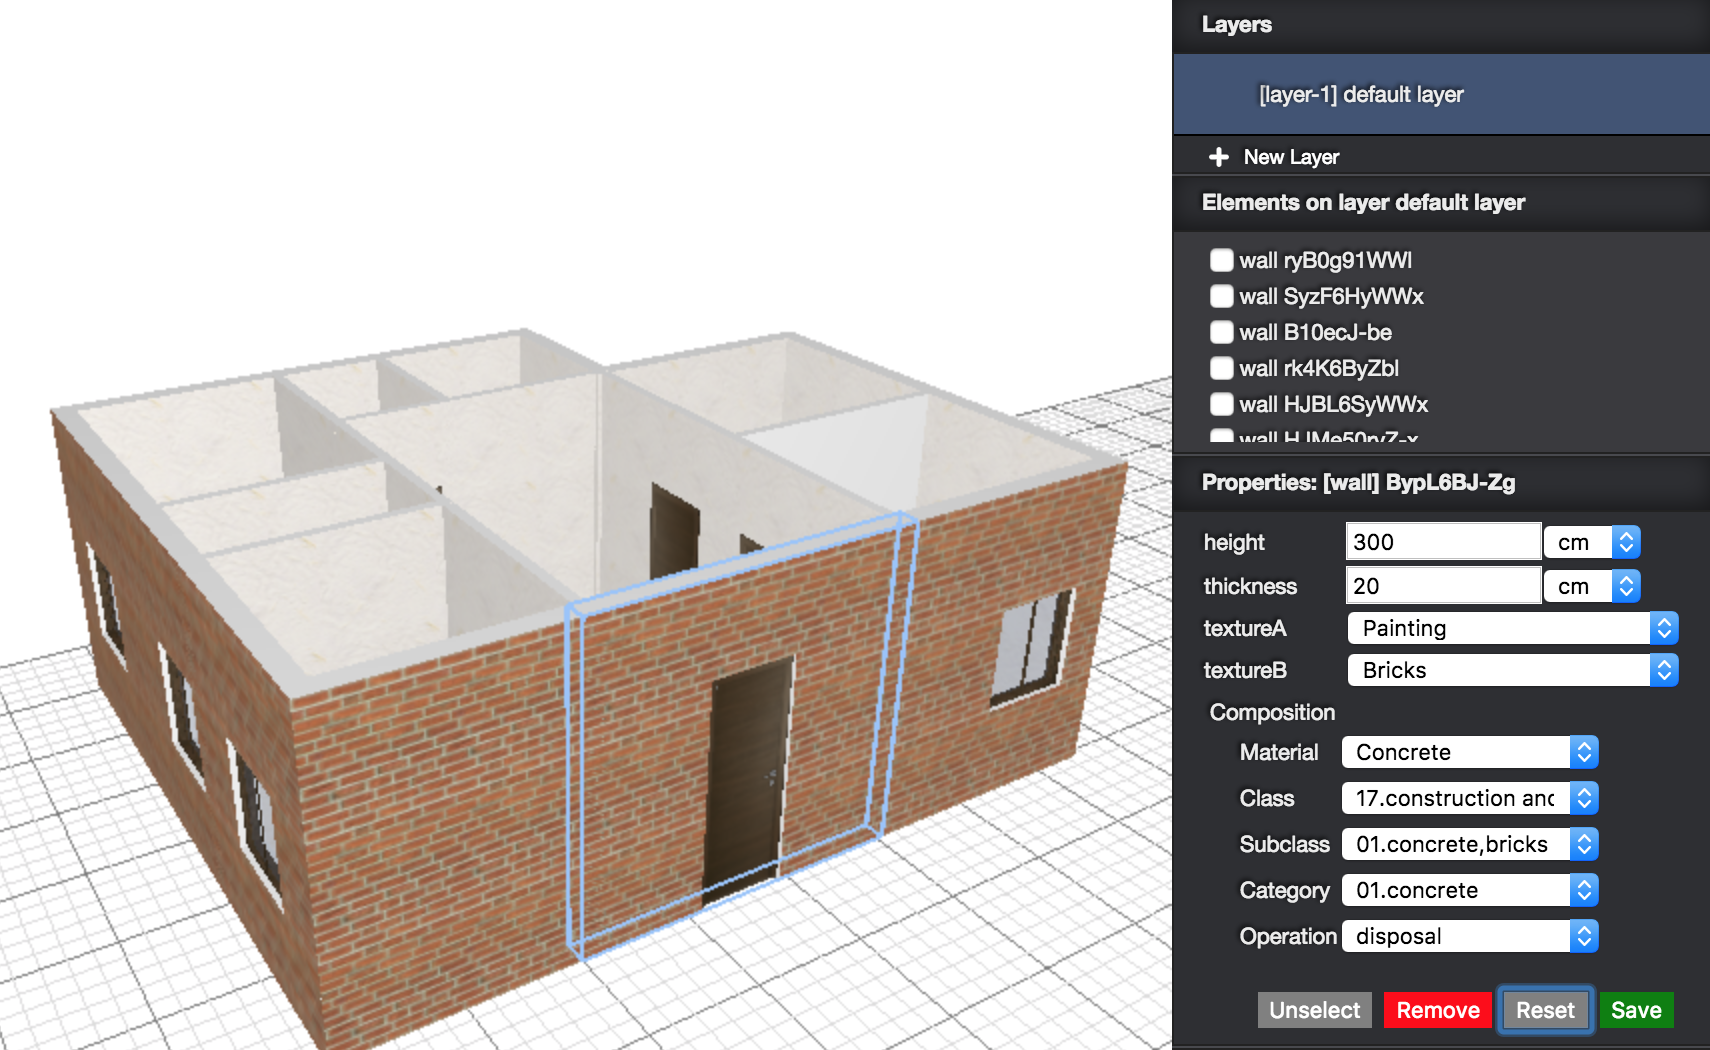
\includegraphics[width=1\linewidth]{images/3d-sel}
   \caption{Vista 3D di un modello per il Deconstruction}
   \label{fig:augmented}
\end{figure}

Un rapporto completo sull'utilizzo BIM come un approccio edificio decostruzione è fornita da~\cite{galic2014bim}.
Uno studio sull'uso del BIM come supporto per la progettazione per Deconstruction è svolta da~\cite{akinade2015waste}.
In questa configurazione, al contrario di ciò di quella usata nel framework \emph{Metior}, la decostruzione deve essere
presa in considerazione a partire dall'inizio della progettazione degli edifici.
\newpage
% In particular, a  geometric modeling of the building allows to identify:
% (a) cost / income resulting from alternatives of recycling / re-using instead of disposal;
% (b) the composition and integration of information useful to the planning of construction activities;
% (c) achievement of the thresholds of reuse / recovery required by the regulations;
% (d) ability to economically compare different options.

% We started by considering the SMARTWaste system~\cite{smartWaste}.
% Their approach allows to derive estimates of the quantities of materials by providing a description of the type of building
% and the area where it was built. With this information, the forms that provide an aggregated representation of the data of
% interest are automatically filled.

% Our approach to deconstruction conversely provides both a geometric modeling of building subsystems and components and a
% semantic annotation with construction materials, like a sort of \emph{simplified} BIM.
% As a matter of fact, our national construction industry is strongly heterogeneous, so that  we need a pretty detailed
% modeling to obtain enough accurate information.
% One vantage point of this approach is an incremental iterative character, where each modeling stage may be followed by
% validation of partial costs.

% A complete report about using BIM as a building deconstruction approach is provided by~\cite{galic2014bim}.
% A study on the usage of BIM as a support for Design for Deconstruction is carried on by~\cite{akinade2015waste}.
% In this setup, on the contrary to what holds for us, deconstruction has to be a major concern starting from the beginning of the building design.


Il framework \emph{Metior} (dal latino: a \emph{misura} o \emph{stima}),
ha come obiettivo superare tali difficoltà, tramite:
\begin{itemize}
  \item la progettazione e realizzazione di un \emph{web service} fornendo un'interfaccia utente semplificata;
  \item memorizzare un database crescente di \emph{Plugin} che rappresentano un modello per le parti di edificio geometricamente più complesse;
  \item utilizzando un motore geometrico estensibile e un Server basato su decenni di ricerca;
  \item offrendo integrazioni semantiche flessibili attraverso la specializzazione di (Industry Foundation Classes~\cite{ifc})
        IFC classi associate ai sottosistemi di costruzione e le parti;
\end{itemize}


% The \emph{Metior} (from Latin: to  \emph{measure} or  \emph{estimate}) project, introduced in this paper,
% is exactly aiming to overcome such difficulties, via (a)~the design and implementation of a \emph{web service}
%   providing a strongly simplified user-interface, designed for quantity surveyors; (b)~storing a growing database
%    of template plugins for more geometrically complex building parts; (c)~using an extensible geometry engine and
%     server based on decades of research; (d)~offering flexible semantic additions via specialization of
%     IFC (Industry Foundation Classes~\cite{ifc}) classes associated to building subsystems and parts.

Considerando ad esempio dei grandi siti che devo subire il processo di decostruzione
sono gestiti dai imprenditori, i quali hanno a disposizione e già utilizzato le competenze e strumenti specifici,
per la maggiorparte delle attività di decostruzione. La maggiorparte dei materiali di scarto prodotto,
sono gestiti da geometri provenienti da aziende di piccole o medie dimensioni o anche da singoli professionisti.
Questo tipo di società necessitano di un sostegno dato da strumenti in cui le complessità,
sia burocratiche che tecniche, devono essere nascoste, anche se correttamente gestite.

% Metior specifically targets quantity surveyors. In fact, although large sites to be deconstructed are operated by main
%  contractors, where skills and specific tools might be widely available and already used, most of deconstruction activities,
%   and hence the largest amount of waste material produced, are managed by quantity surveyors from small or medium companies
%   --- or even by single professionals. Such kind of firms may need to be supported with tools where the complexity,
%   both bureaucratic and technical, have to be hidden although correctly managed.
